\section{Roboterfunktionen}
\subsection{Grosser Roboter}

\begin{frame}
	\frametitle{Supportrad}
	
\end{frame}

\begin{frame}
	\frametitle{Walze und Leitplanke}
	
\end{frame}

\begin{frame}
	\frametitle{Riemen und Abstreifvorrichtung}
	
\end{frame}

\begin{frame}
	\frametitle{Schussmechanismus}
	
\end{frame}

\subsection{Kleiner Roboter}

\begin{frame}
	\frametitle{Modulaufnahme}
	Mithilfe eines Scherenzugs sollten die \textit{Lunar Modules} aus den Raketen gezogen werden.
	Dieses Konzept funktionierte nicht wunschgemäss und wurde deshalb durch einen Greifer und einen Pressfinger ersetzt.\\
	
	\begin{figure}
		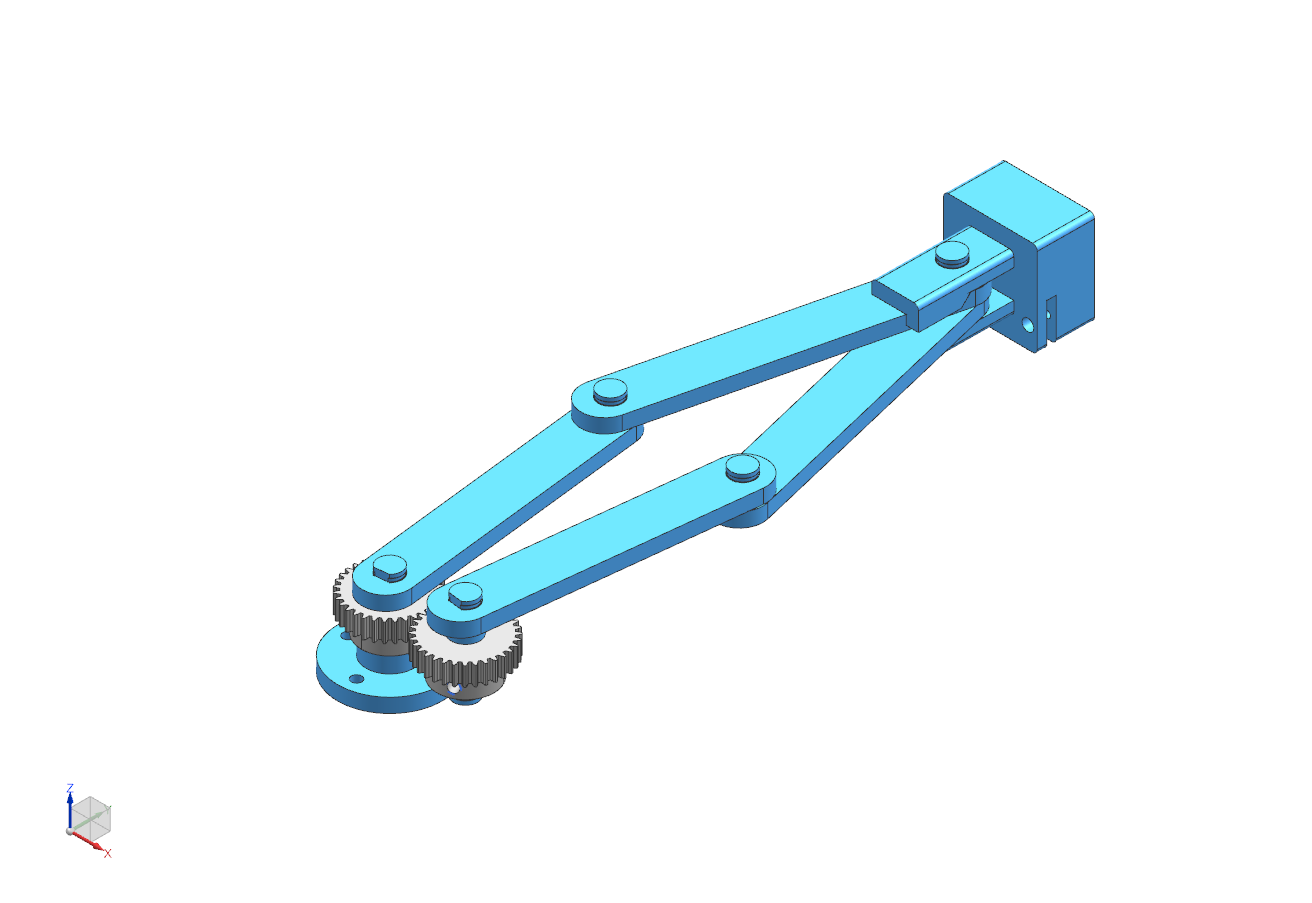
\includegraphics[height = 3 cm]{../images/presentation/kleinerRoboter/Schere.png}
		\hspace{1em}
		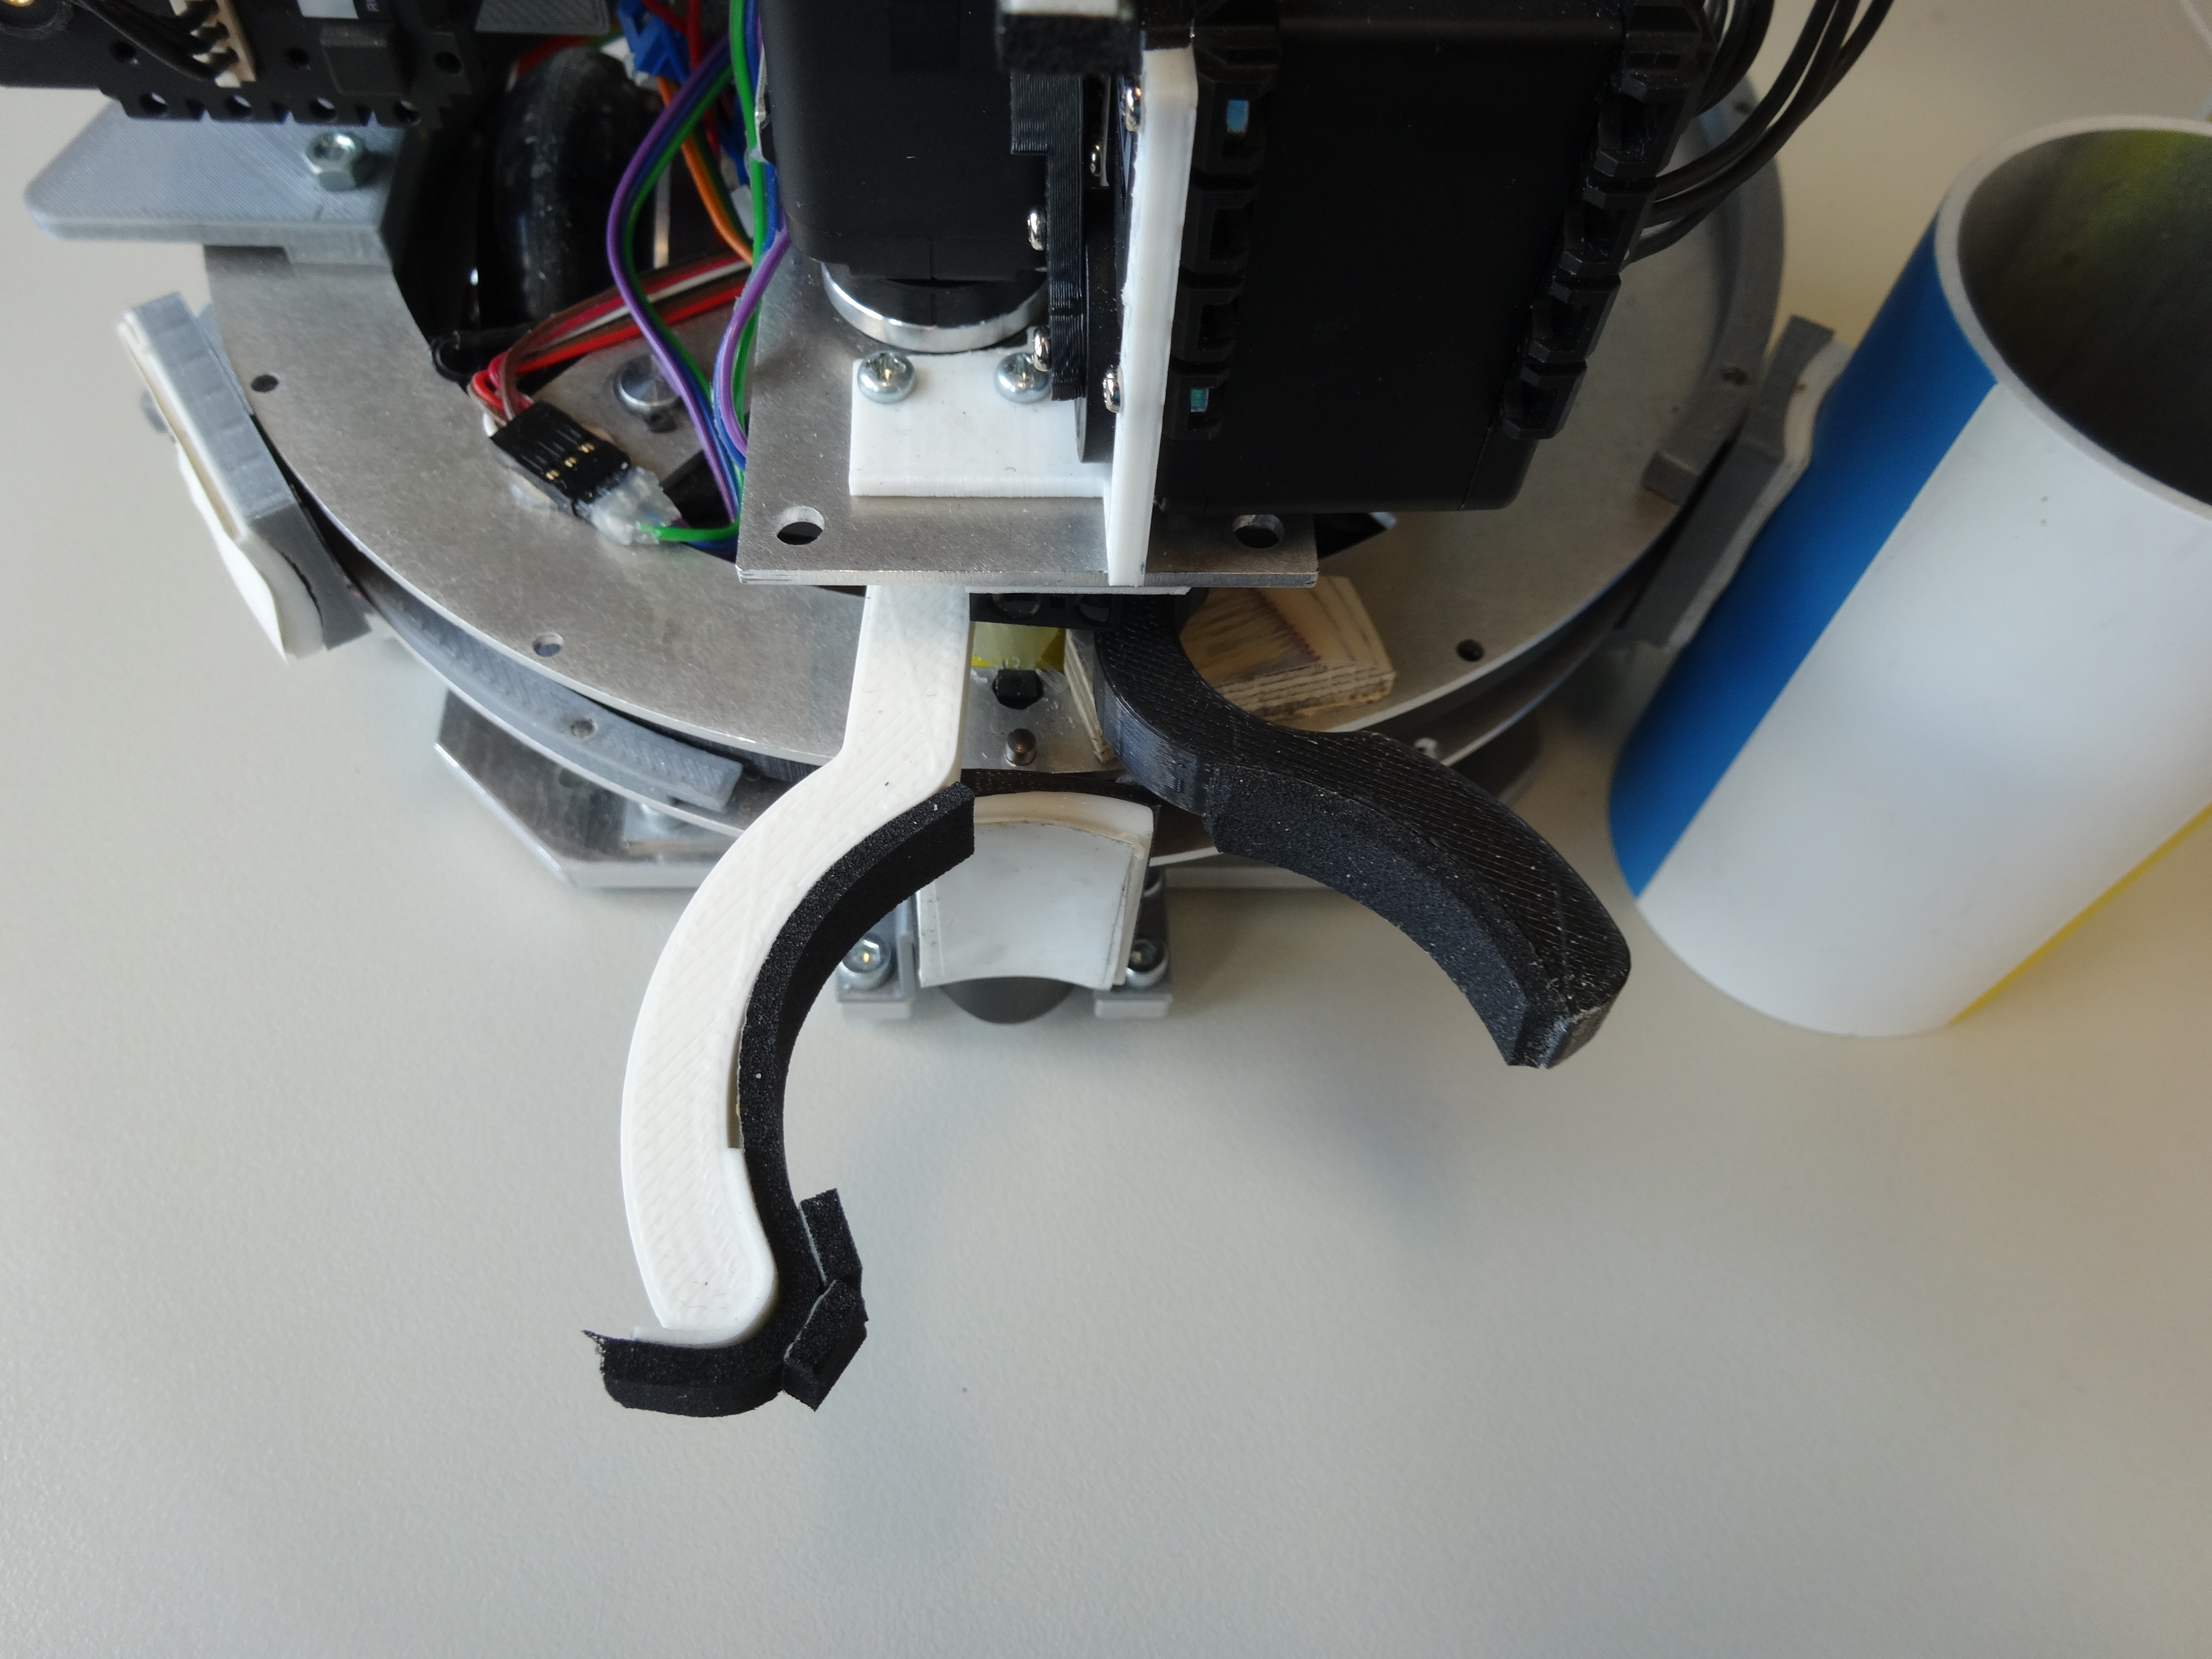
\includegraphics[height = 3 cm]{../images/presentation/kleinerRoboter/Greifer.jpg}
		\hspace{2em}
		\includegraphics[angle = 90, height = 3 cm]{../images/presentation/kleinerRoboter/Pressfinger.jpg}
	\end{figure}
\end{frame}

\begin{frame}
	\frametitle{Ring}
	Die \textit{Lunar Modules} haften während dem Transport an den Klebestellen des Rings.
	Durch drehen des Rings werden sie gekippt und abgestreift.
	\begin{figure}
		\centering
		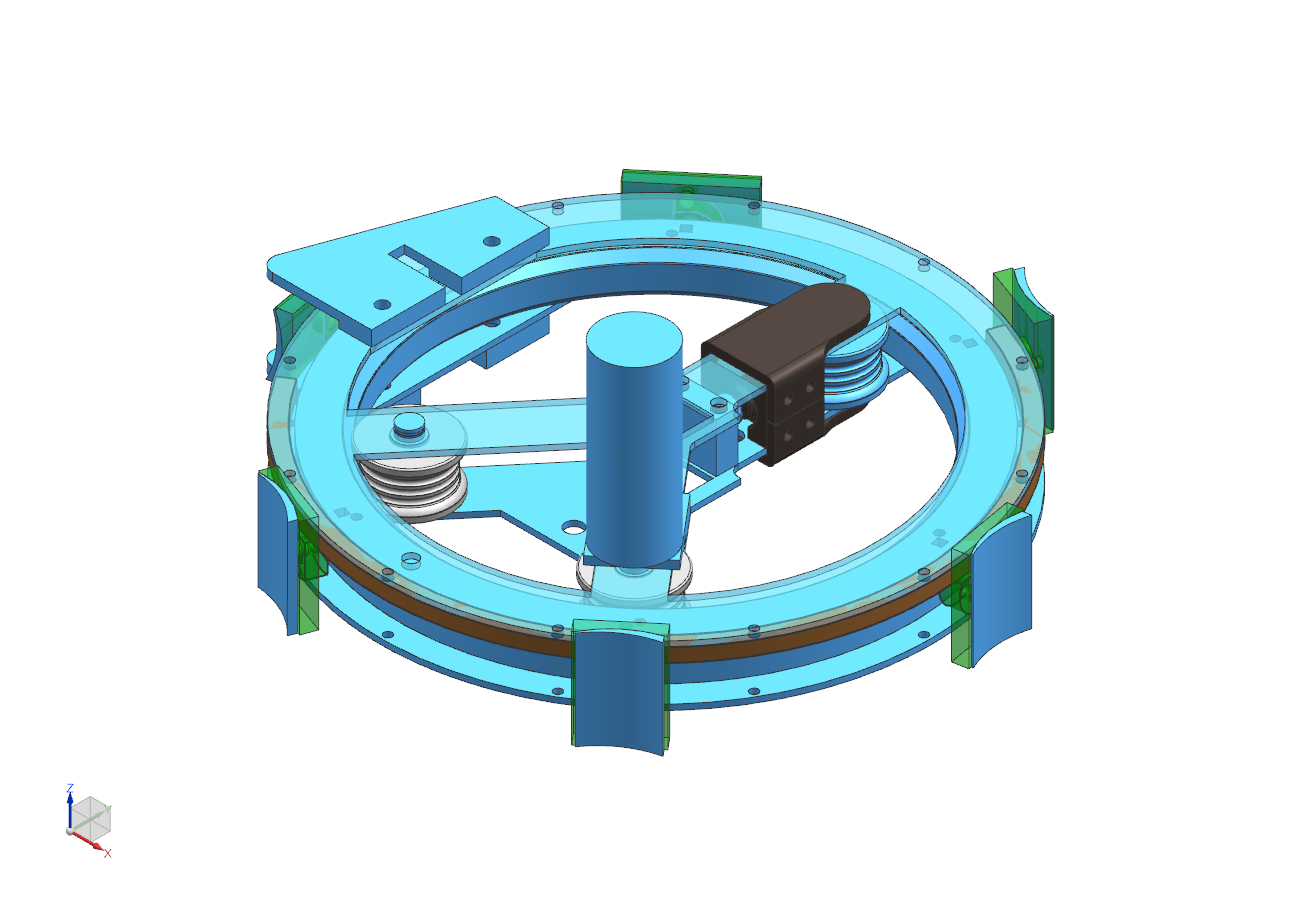
\includegraphics[height = 4 cm]{../images/presentation/kleinerRoboter/Ring.png}
	\end{figure}
\end{frame}

\begin{frame}
	\frametitle{Drehmechanismus}
	Ein Arm mit einem Farbsensor und einem Rad kann ausgeklappt werden um \textit{Lunar Modules} zu drehen oder zu verschieben.
	\begin{figure}
		\centering
		\includegraphics[height = 4 cm]{../images/presentation/kleinerRoboter/Drehen.jpg}
	\end{figure}
\end{frame}